\section{Scenarios and Tasks}
\label{sec:evaluation-scenarios}

The test is composed by four tasks: each task has multiple goals defined as 'task rationale'; the first two tasks start from an empty project and require users to model the described experience from scratch, the last two tasks instead are presented with an already-modeled experience in which users are required to perform some changes or complete them to have a correctly designed experience.
The list of task rationales R1--R12 is described below and \autoref{table:evaluation-task-rationale} shows which task is based on these objectives.
\begin{itemize}
    \item[R1]Add multiple state and action nodes
    \item[R2]Add action and state tags
    \item[R3]Link states to actions and vice versa
    \item[R4]Keep coherent identifiers when referring to the same object
    \item[R5]Change tag properties
    \item[R6]Edit labels
    \item[R7]Add two conditional action nodes
    \item[R8]Link back to an initial state
    \item[R9]Add more than one object to the same node
    \item[R10]Add more than one tag to the same object
    \item[R11]Edit the recipe name
    \item[R12]Save the modeled experience
\end{itemize}

\begin{table}[h!]
\centering
\begin{tabular}{|l|c|c|c|c|c|c|c|c|c|c|c|c|} 
\cline{2-13}
\multicolumn{1}{l|}{} & \multicolumn{1}{l|}{R1} & \multicolumn{1}{l|}{R2} & \multicolumn{1}{l|}{R3} & \multicolumn{1}{l|}{R4} & \multicolumn{1}{l|}{R5} & \multicolumn{1}{l|}{R6} & \multicolumn{1}{l|}{R7} & \multicolumn{1}{l|}{R8} & \multicolumn{1}{l|}{R9} & \multicolumn{1}{l|}{R10} & \multicolumn{1}{l|}{R11} & \multicolumn{1}{l|}{R12}  \\ 
\hline
\textit{Task 1}       & x & x & x & x &   &   &   &   &   &    &    &     \\ 
\hline
\textit{Task 2}       & x & x & x & x & x & x &   &   &   &    &    &     \\ 
\hline
\textit{Task 3}       &   & x &   & x & x & x & x & x &   &    &    &     \\ 
\hline
\textit{Task 4}       &   &   &   &   &   &   &   &   & x & x  & x  & x   \\
\hline
\end{tabular}
\caption{Task rationales by task.}
\label{table:evaluation-task-rationale}
\end{table}


\subsection*{Task 1}
    \textit{Instructions:} 
\begin{enumerate}
    \item Given the initial \textit{State Node} in the diagram, place a 3D Model inside it, chosen from the list of Elements on the left.
        \begin{itemize}
        \item[-] add a \textit{State Tag} to make it \textbf{Visible}.
        \end{itemize}
    \item Insert an \textit{Action Node} containing the 3D Model element and the \textit{Action Tag} \textbf{Tap} on the 3D Model.
    \item Connect the previously made \textit{State Node} to the \textit{Action Node}.
    \item Add a new \textit{State Node} and link the last \textit{Action Node} to it. Within this new \textit{State Node} add a 2D Text and add a \textit{State Tag} to make it \textbf{Visible}.
    \item Change the ID of the 3D Model editing the little dark blue square containing the ID number to make it equal to the previous ID of the 3D Model.
\end{enumerate}
The solution to this task is shown in \autoref{fig:task1-sol}.
\begin{figure}[h]
    \centering
    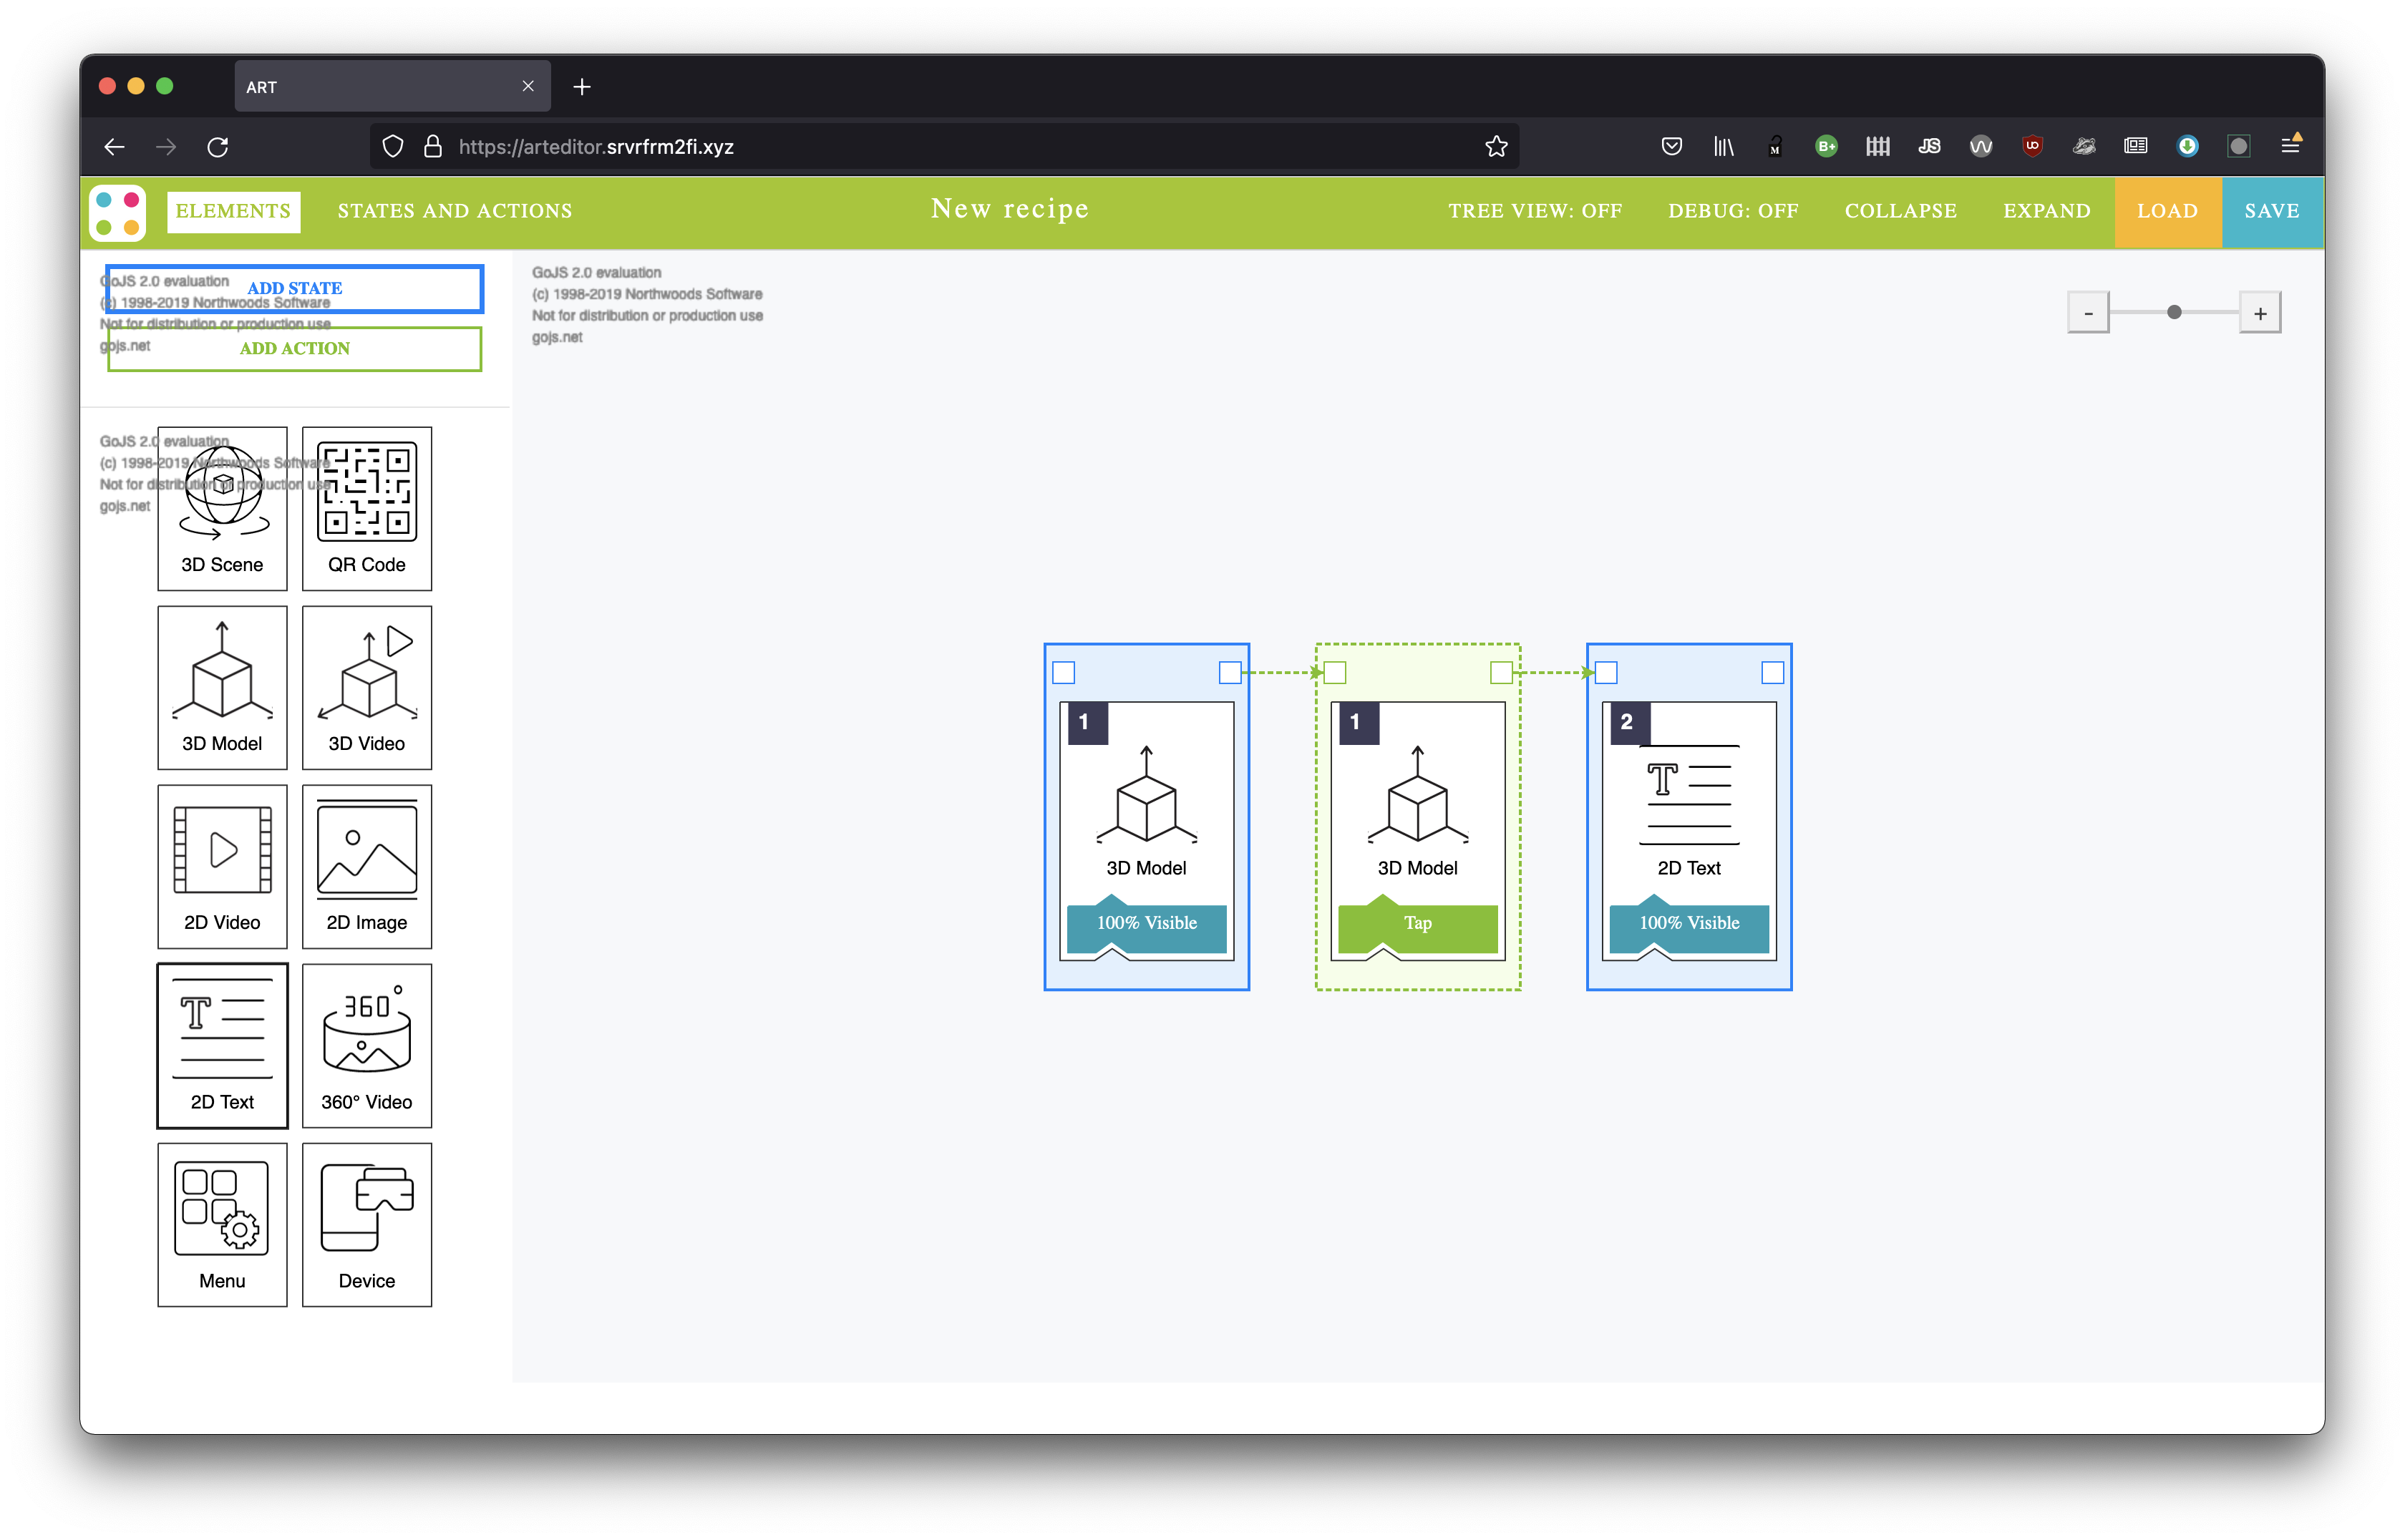
\includegraphics[width=\linewidth]{Figures/Evaluation/Tasks/task1-sol.png}
    \caption{Solution to task 1}
    \label{fig:task1-sol}
\end{figure}

\subsection*{Task 2}
\textit{Instructions:} 
\begin{enumerate}
    \item Given the initial \textit{State Node} in the diagram, place a 2D Video inside it
        \begin{itemize}
            \item[-] add the \textit{State Tag} \textbf{Visible} to it.
        \end{itemize}
    \item Add an \textit{Action Node} (with the 2D Video inside) linked to the last created \textit{State Node} and model its final \textit{State Node} as: when the user \textbf{Taps} on the video it becomes \textbf{On Play}.
    \item Change the 2D Video Visible \textit{State Tag} options in:
        \begin{itemize}
            \item[-] 3 seconds fade in animation
            \item[-] after 2 seconds.
        \end{itemize}
    \item Change the \textit{Label Name} in “First Recording”.
    \item Change the 2D Video \textbf{On Play} \textit{State Tag} options in: Loop enabled.
    \item Sync IDs and \textit{Label Name}, they must be coherent in the whole sequence.
\end{enumerate}
The solution to this task is shown in \autoref{fig:task2-sol}.
\begin{figure}[h]
    \centering
    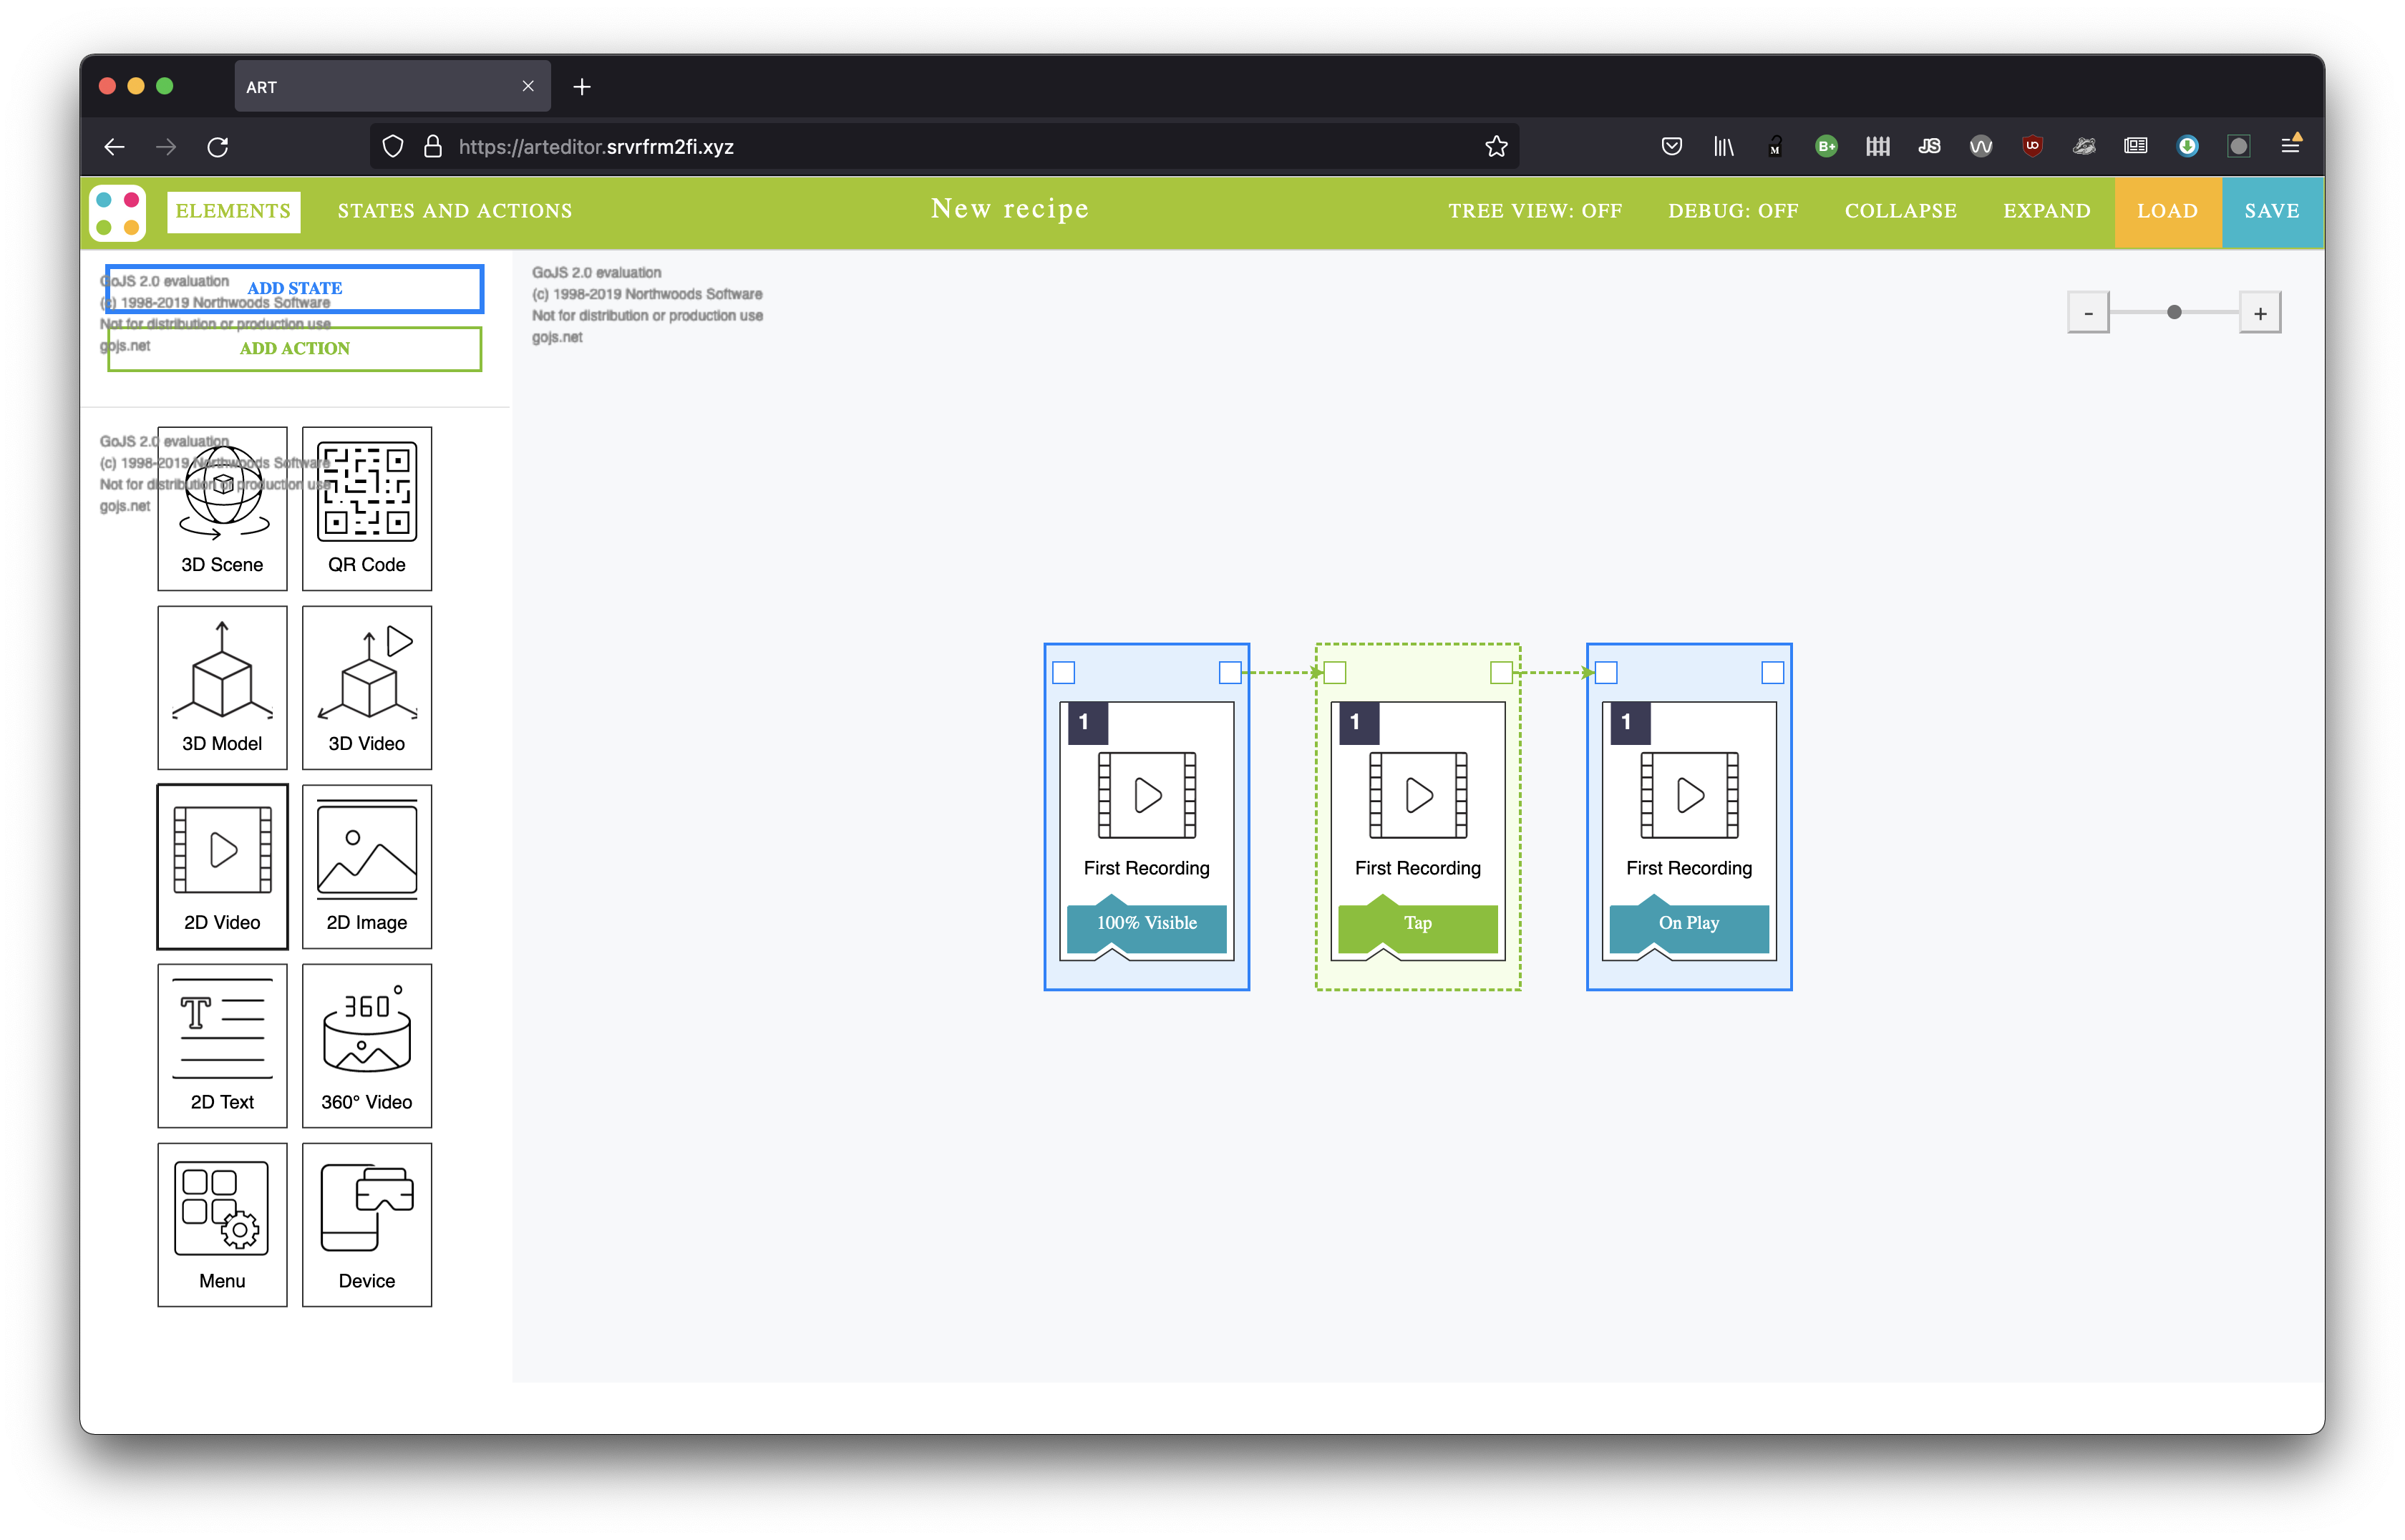
\includegraphics[width=\linewidth]{Figures/Evaluation/Tasks/task2-sol.png}
    \caption{Solution to task 2}
    \label{fig:task2-sol}
\end{figure}

\subsection*{Task 3}
\textit{Instructions:} 
The experience already modeled in the diagram (see \autoref{fig:task3-pre}) describes a scenario with two scenes:
Scene 1 contains a 2D Video (with ID 5), Scene 2 contains a 3D Video (with ID 4).
The scenes are initially \textbf{Hidden} and become \textbf{Visible} after the user enters in their proximity zone.
\begin{enumerate}
    \item When 3D Scene1 becomes \textbf{Visible} add, to the 2D Video, the \textit{State Tag} \textbf{Visible} and set its opacity to 90\%.
    \item To the last \textit{State Node} containing the 3D Scene 1 add two distinct \textit{Action Nodes} (respectively with the 2D Video and the 3D Scene) starting from the last created \textit{State Node} and model their final \textit{State Nodes}:
        \begin{itemize}
            \item[-]If the user \textbf{Taps} on the video it becomes \textbf{On Play}.
            \item[-]If the user exits (\textbf{Proximity Out}) from Scene 1, the 3D Scene becomes again \textbf{Hidden}, after 20 seconds, so link this \textit{Action Node} to the initial \textit{State Node} where Scene 1 is \textbf{Hidden}.
        \end{itemize}
    \item Change the \textbf{On Play} settings of the 3D Video with ID 4 to make it playing in loop.
    \item The IDs of the elements must be coherent in the whole sequence.
\end{enumerate}
The solution to this task is shown in \autoref{fig:task3-sol}.
\begin{figure}[h]
    \centering
    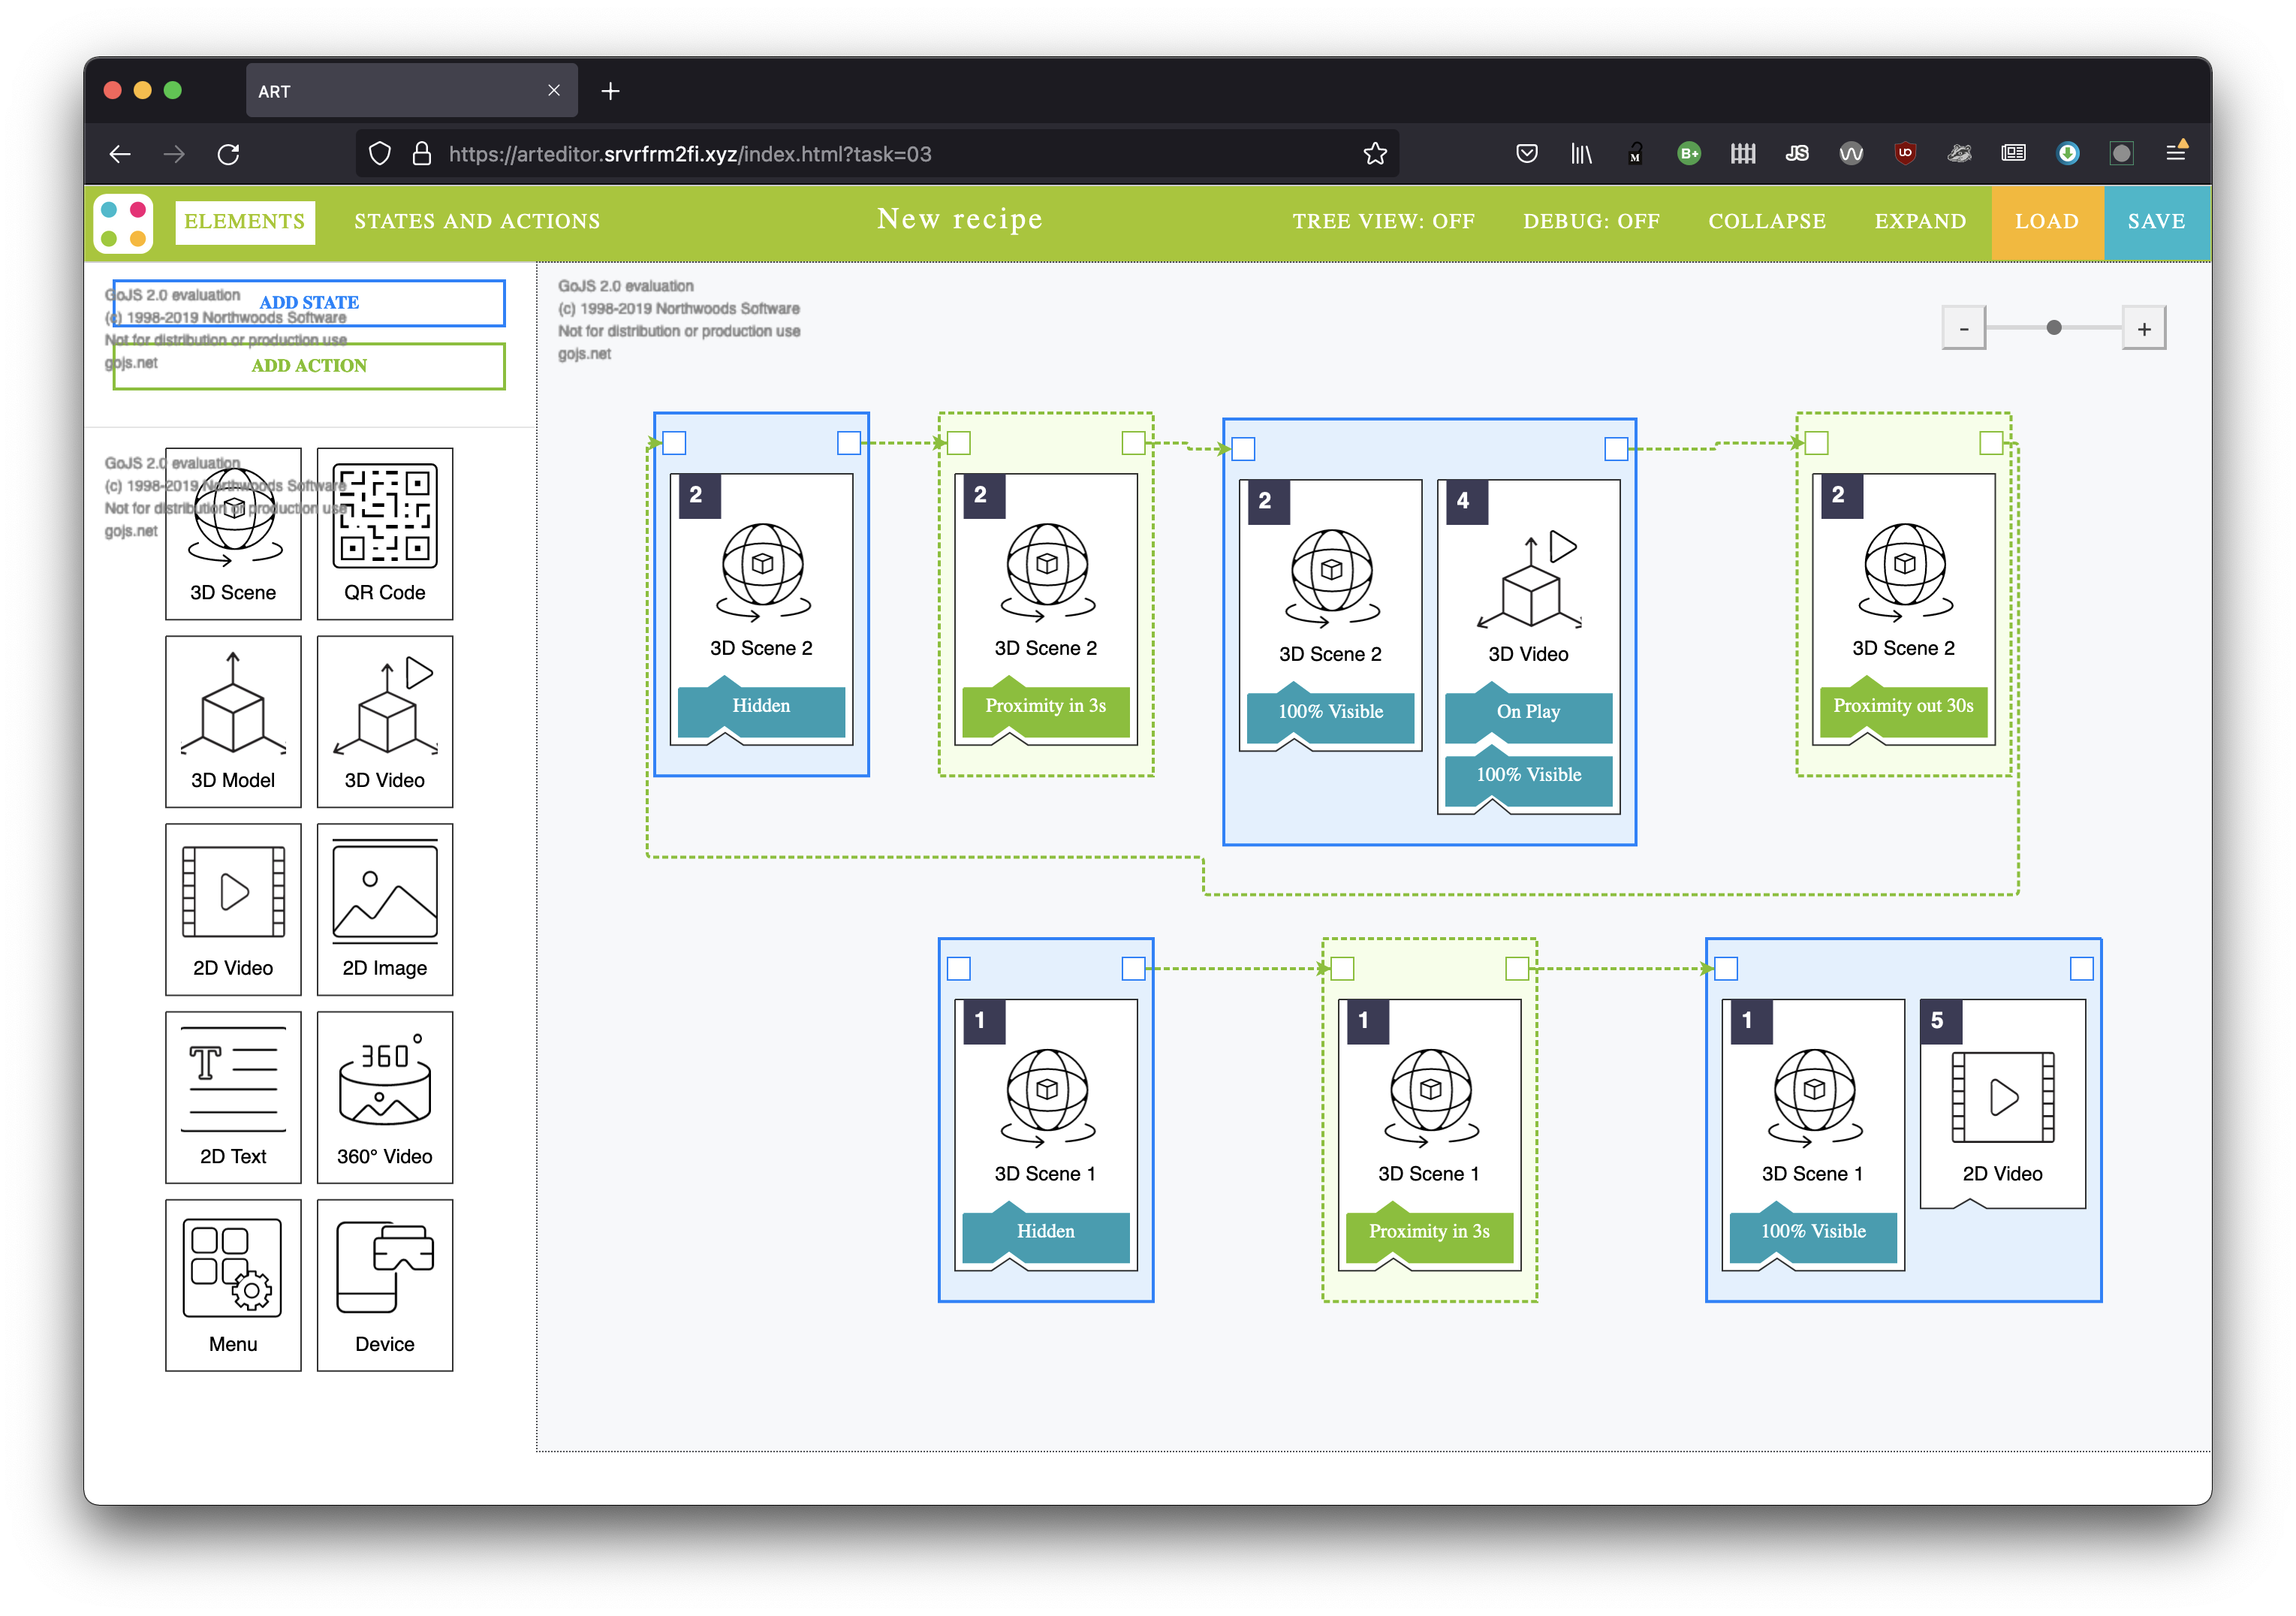
\includegraphics[width=\linewidth]{Figures/Evaluation/Tasks/task3-pre.png}
    \caption{Task 3}
    \label{fig:task3-pre}
\end{figure}

\begin{figure}[h]
    \centering
    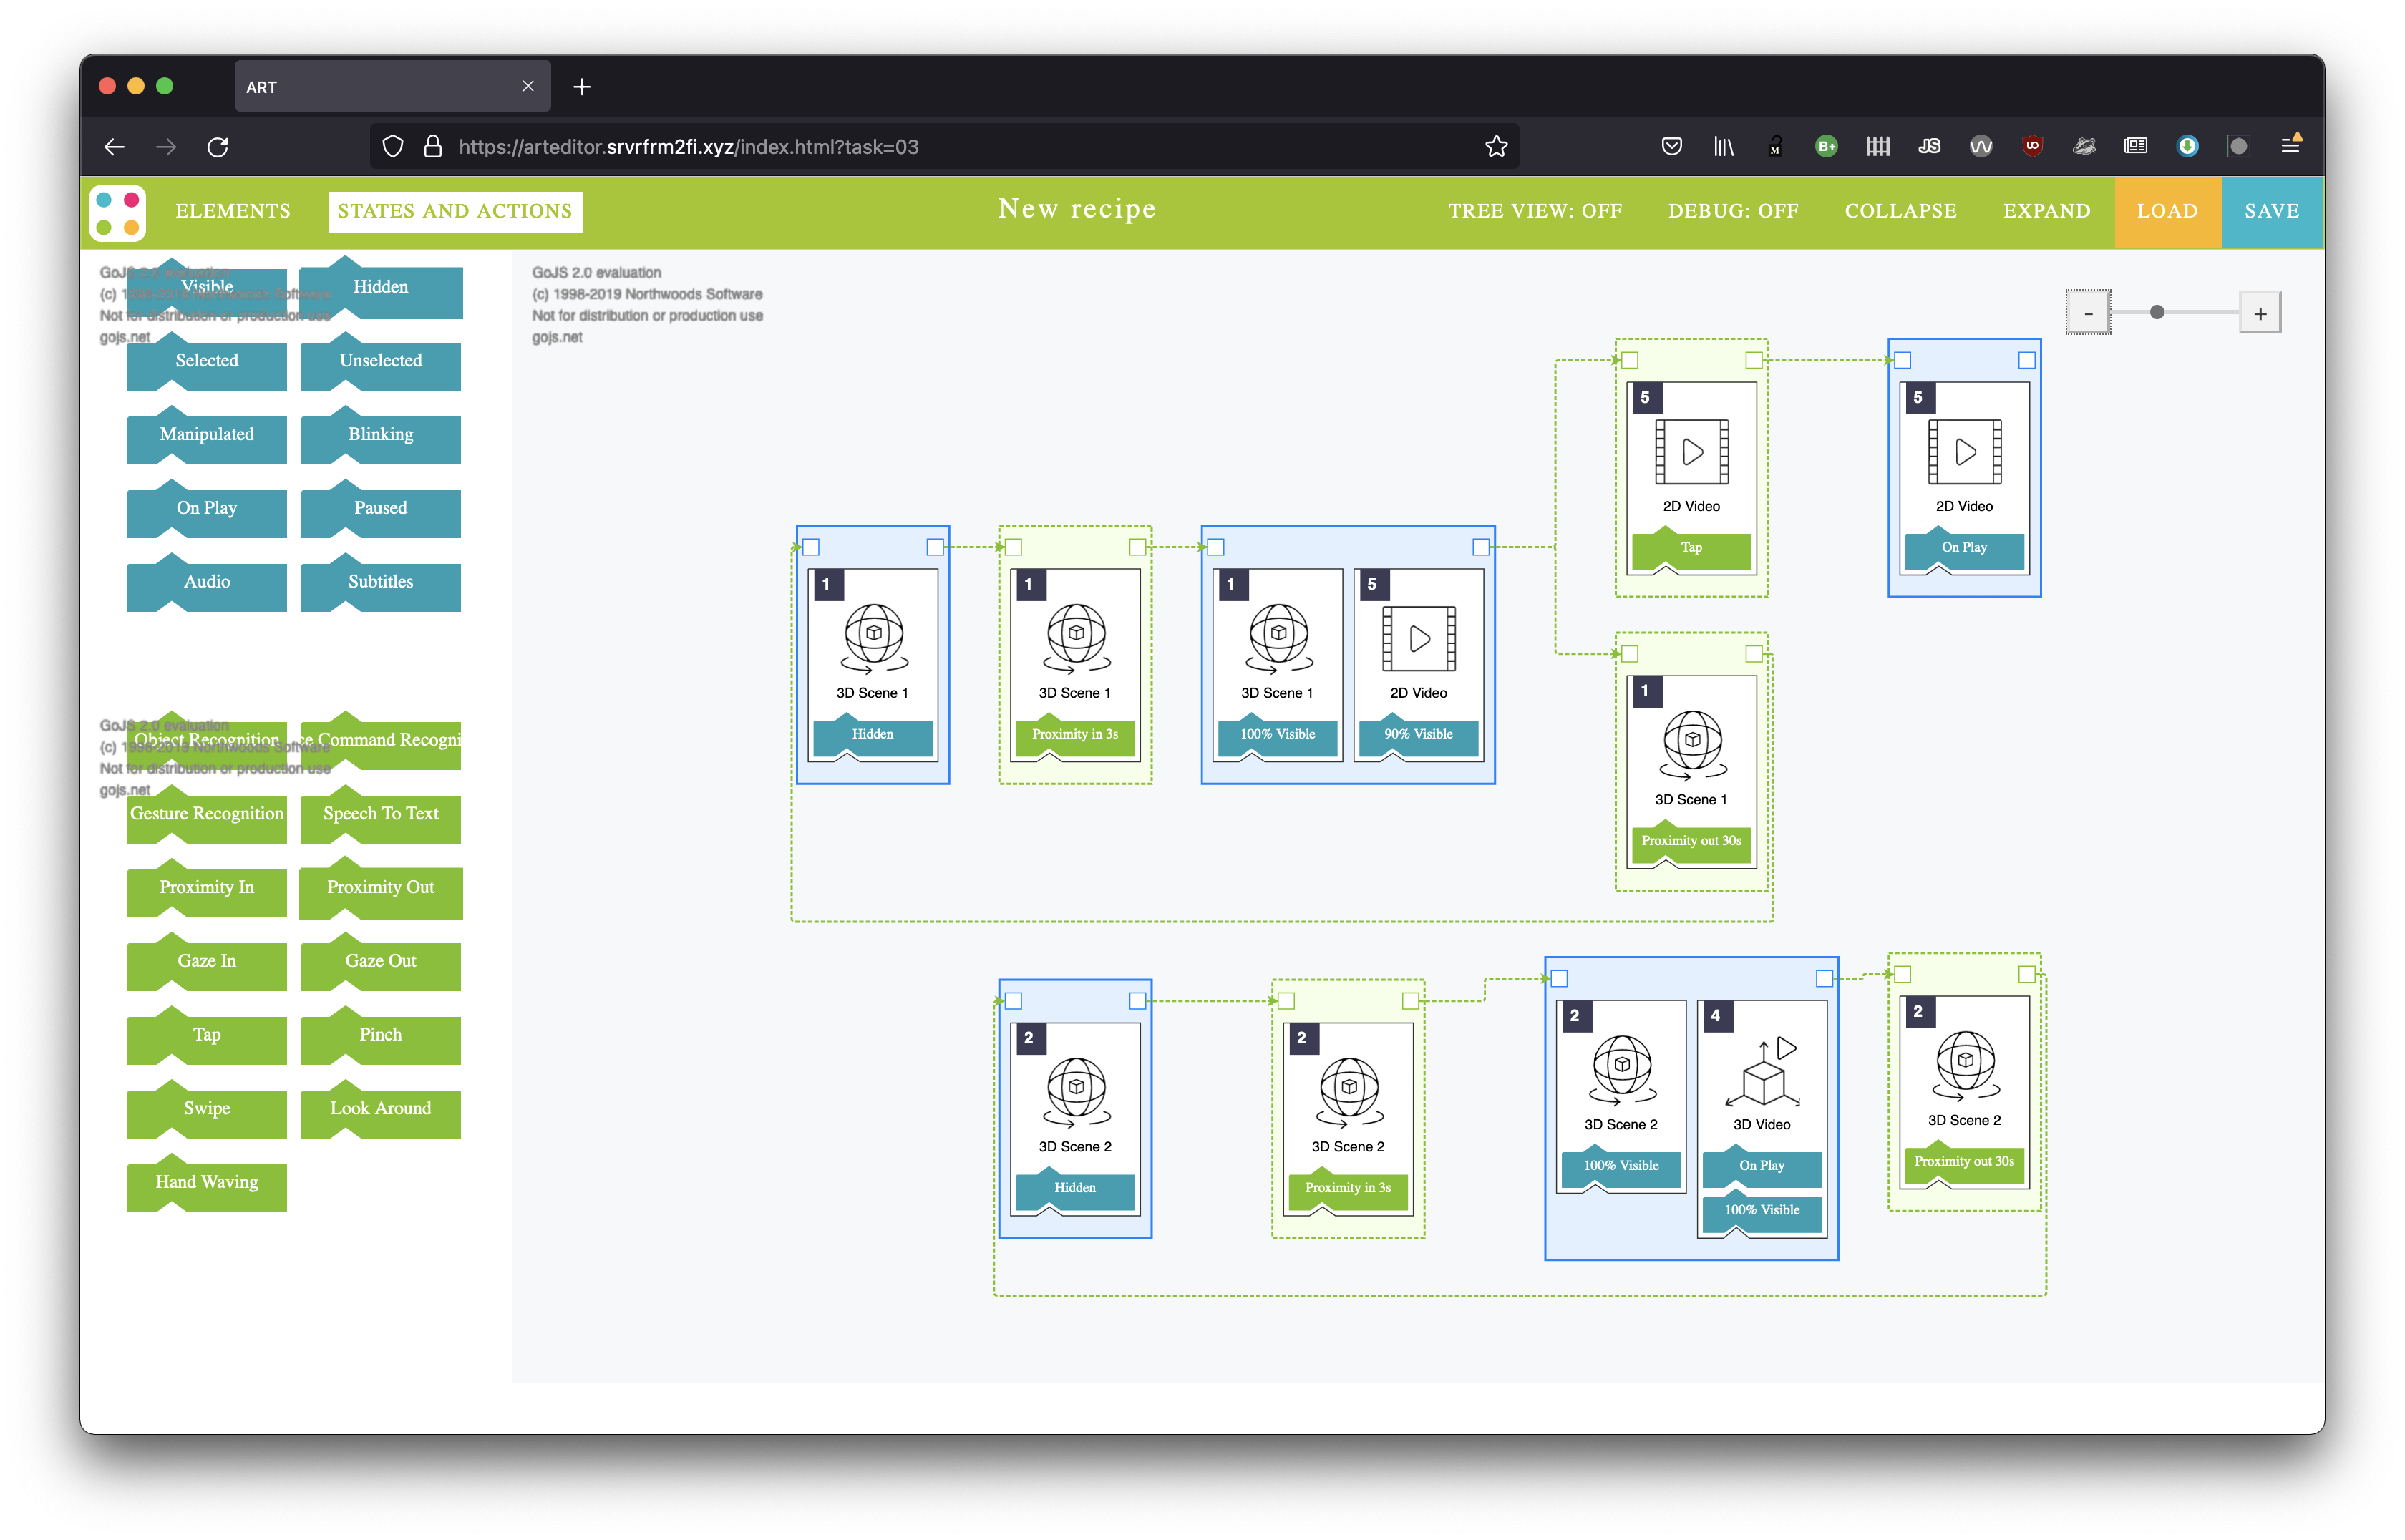
\includegraphics[width=\linewidth]{Figures/Evaluation/Tasks/task3-sol.png}
    \caption{Solution to task 3}
    \label{fig:task3-sol}
\end{figure}


\subsection*{Task 4}
\textit{Instructions:} 
Given the experience already modeled in the diagram (\autoref{fig:task4-pre}):
\begin{itemize}
    \item[-] Change the name of the Canva from “New recipe” to “Task 4”
\end{itemize}
Model the following interactions in Scene 1:
\begin{itemize}
    \item[-]When a \textbf{Tap} action is performed on the Menu (with ID 5), the 3D Video ends in a state with its \textbf{Audio} set to \textbf{Off} and its \textbf{Subtitles} set to \textbf{On}.
\end{itemize}
Model the following interactions in Scene 2:
\begin{enumerate}
    \item Inside the empty \textit{Action Node}, after the 3D Model becomes \textbf{Selected}, add the action by the user that goes away (\textbf{Proximity Out}) from the 3D Model and getting closer to (\textbf{Proximity In}) the 3D Video.
    \item In the final state (from the last modeled action) the 3D Video starts \textbf{Blinking} while the 3D Model becomes \textbf{Hidden}.
    \item[*] The IDs of the elements must be coherent in the whole sequence.
\end{enumerate}
At the end, SAVE the experience “Task 4”. \\
The solution to this task is shown in \autoref{fig:task4-sol}.
\begin{figure}[h]
    \centering
    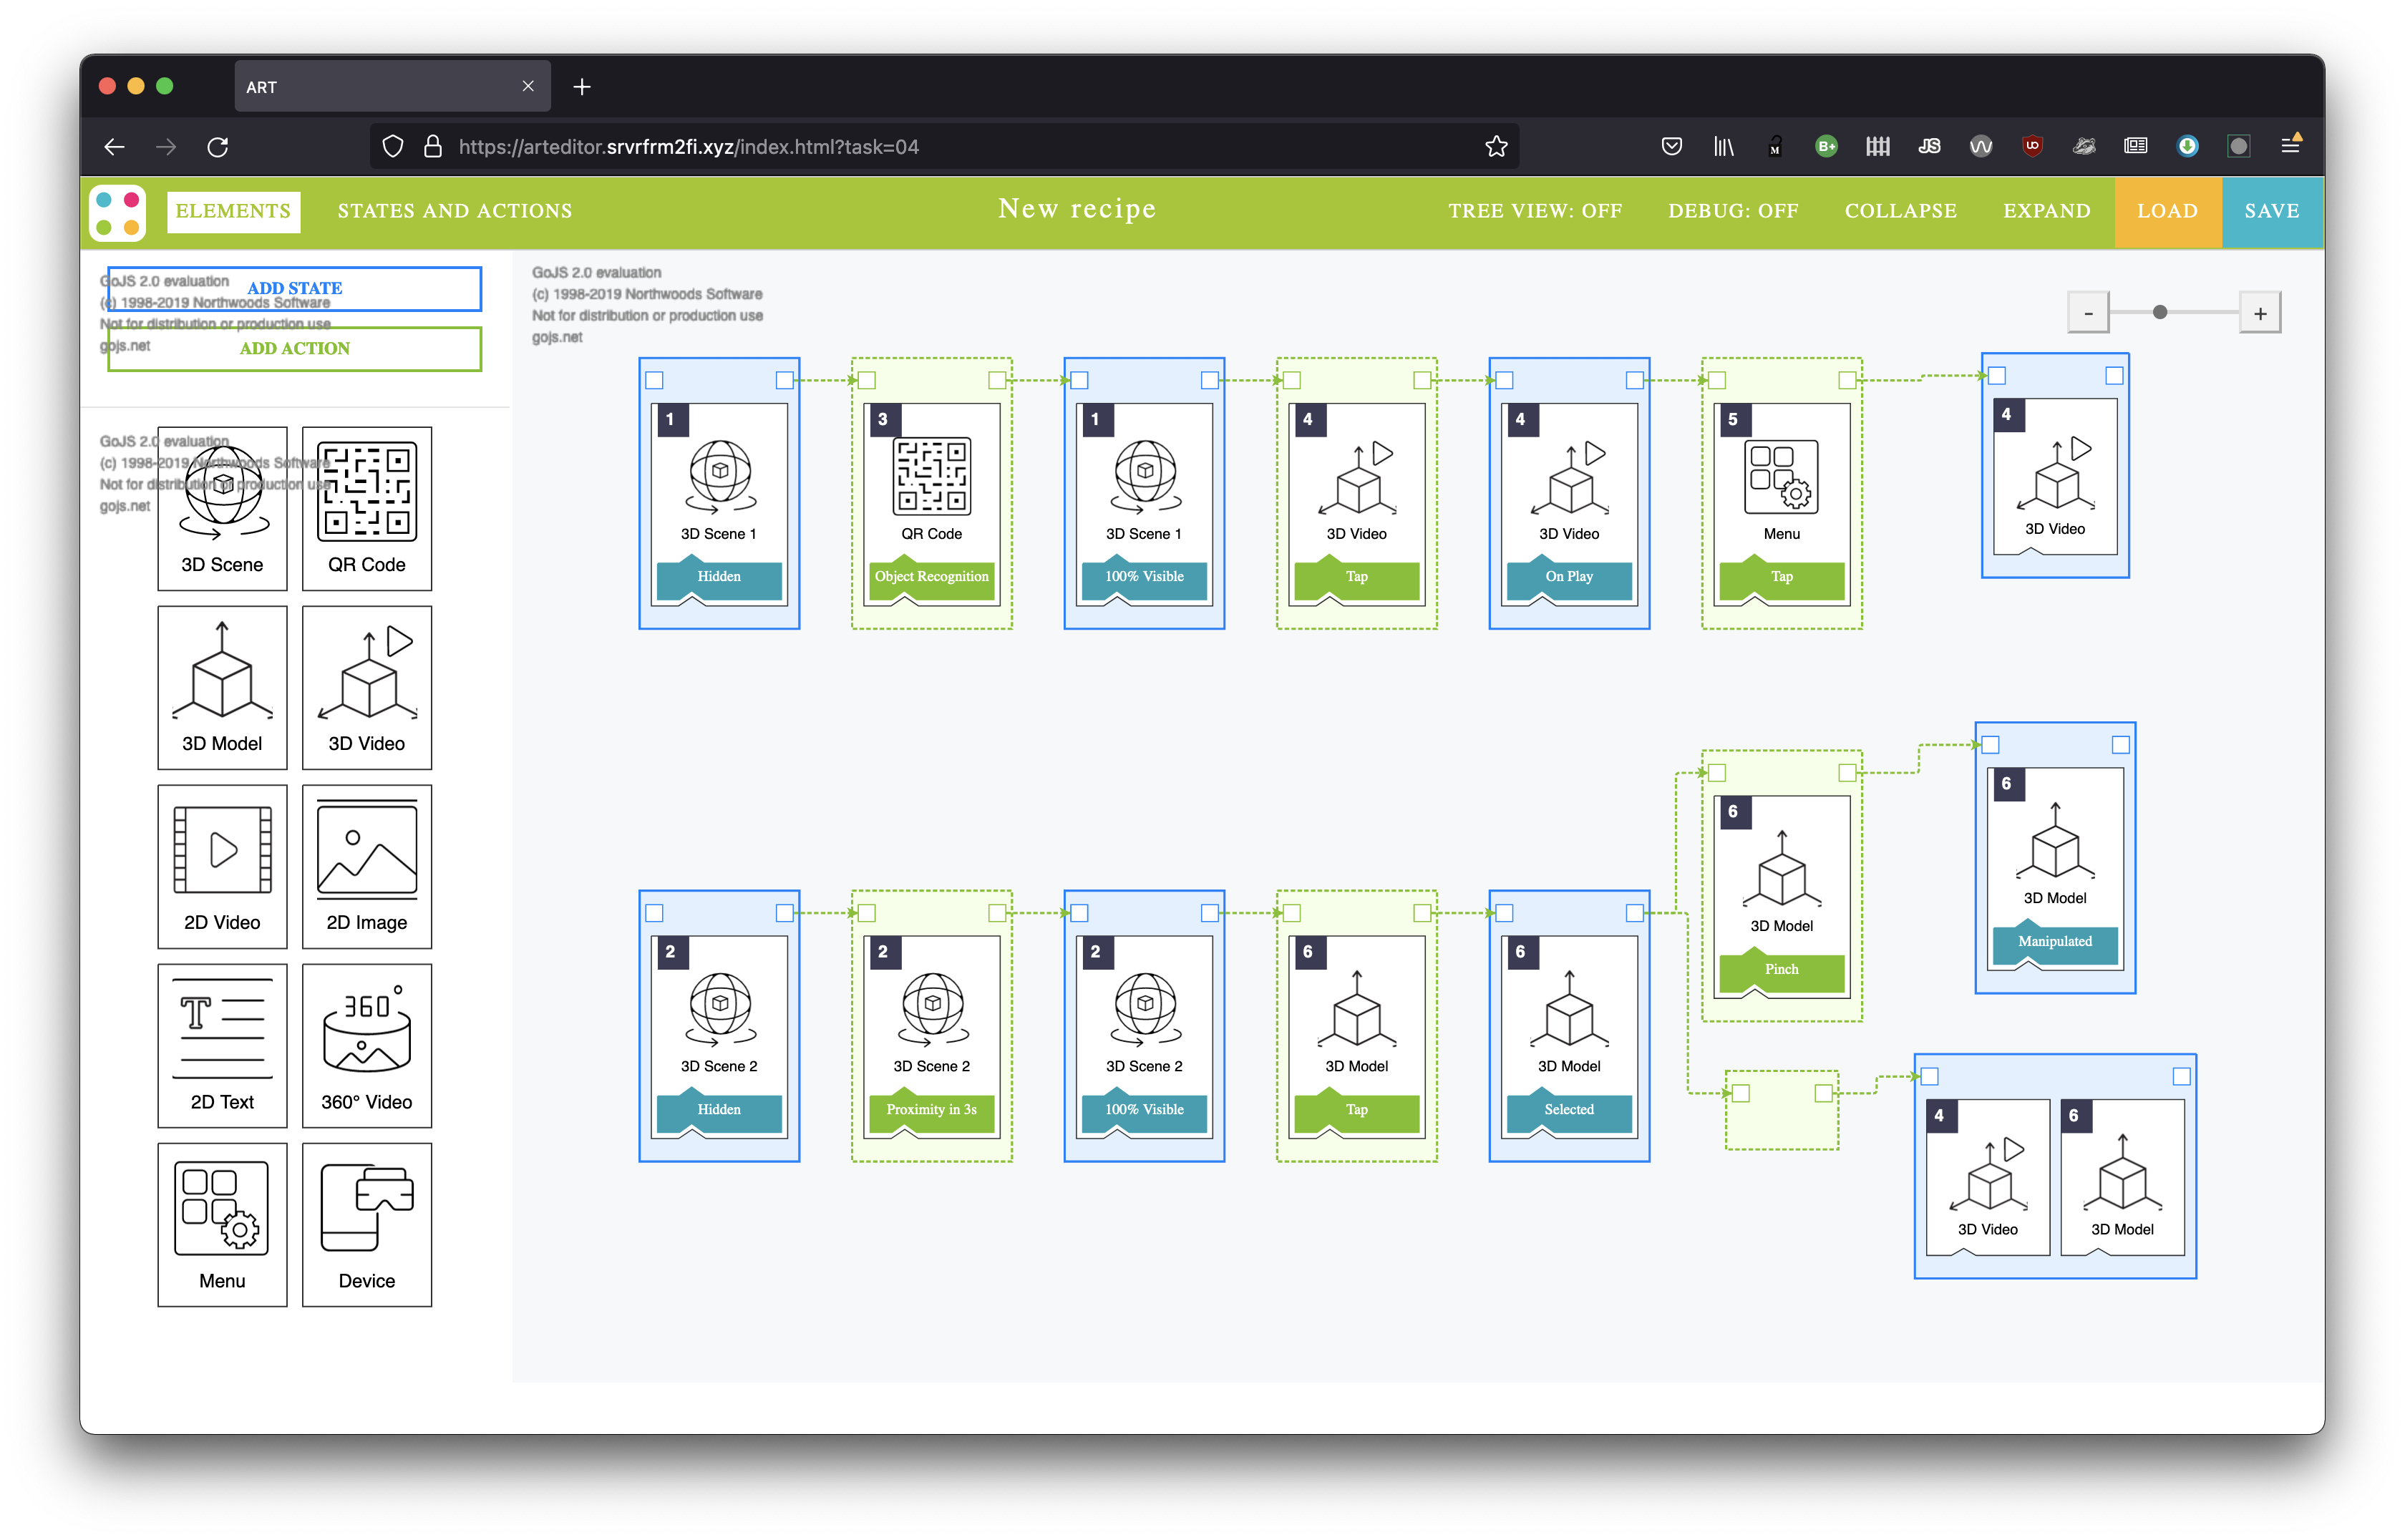
\includegraphics[width=\linewidth]{Figures/Evaluation/Tasks/task4-pre.png}
    \caption{Task 4}
    \label{fig:task4-pre}
\end{figure}

\begin{figure}[h]
    \centering
    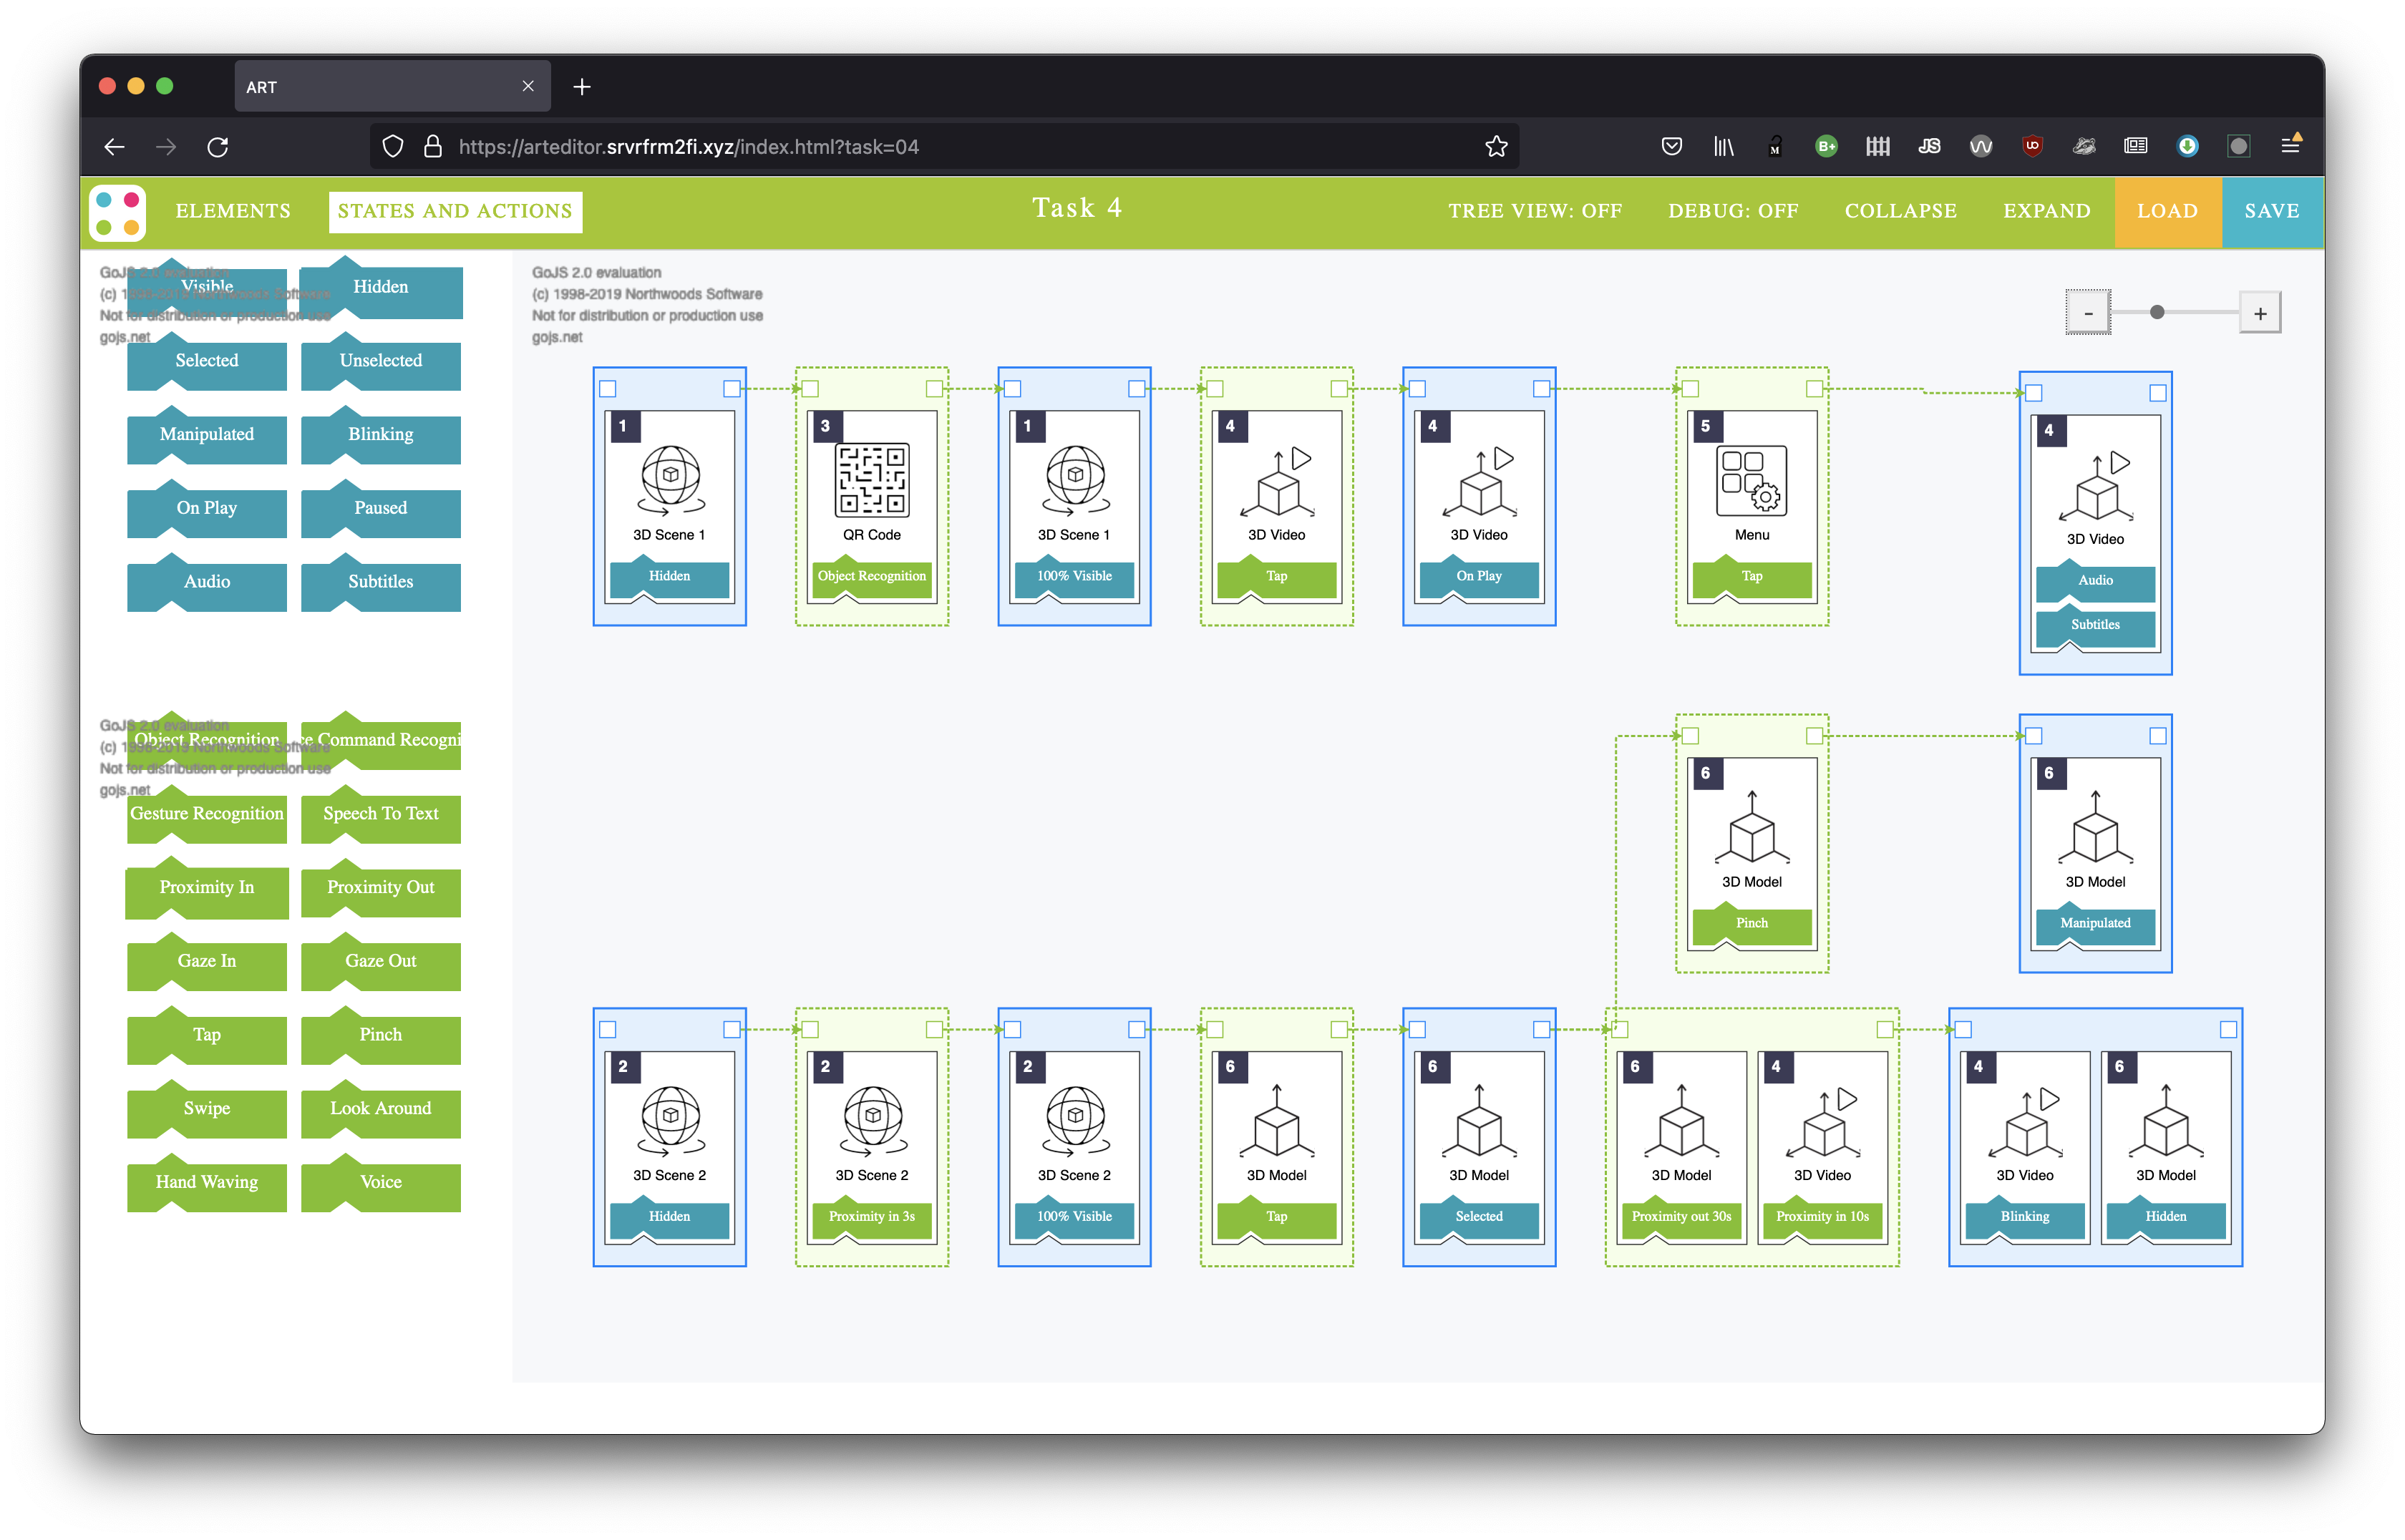
\includegraphics[width=\linewidth]{Figures/Evaluation/Tasks/task4-sol.png}
    \caption{Solution to task 4}
    \label{fig:task4-sol}
\end{figure}